
El presente proyecto consiste en la implementación de una \textbf{mini plataforma de video streaming P2P con microservicios}, cuyo objetivo es permitir que diferentes nodos intercambien fragmentos de video de manera distribuida, sin depender de un único servidor central para el envío de datos.

\subsection*{Planteamiento del Problema}
Las plataformas de streaming tradicionales dependen de un servidor central que entrega el contenido directamente a cada usuario. Esto genera un cuello de botella cuando muchos usuarios solicitan el mismo video.  
En este proyecto se busca aprovechar el \textbf{modelo P2P} para que cada nodo no solo consuma, sino que también comparta fragmentos con otros, reduciendo la carga central.

\subsection*{Estructura de la Solución}
La solución se basa en tres elementos clave:
\begin{enumerate}
    \item \textbf{Servicio Central (Registry Service)}: Registra nodos y mantiene un mapeo de qué fragmentos posee cada uno.
    \item \textbf{Nodos P2P}: Almacenan y comparten fragmentos de video, comunicándose directamente para transferir datos.
    \item \textbf{Sistema Pub/Sub con Redis}: Notifica a los nodos cuando hay nuevos fragmentos disponibles.
\end{enumerate}

\subsection*{Diagrama de Arquitectura}
Diseño del esquema general del sistema, incluyendo el servicio central, los nodos P2P y el canal de comunicación Pub/Sub.

\begin{center}
    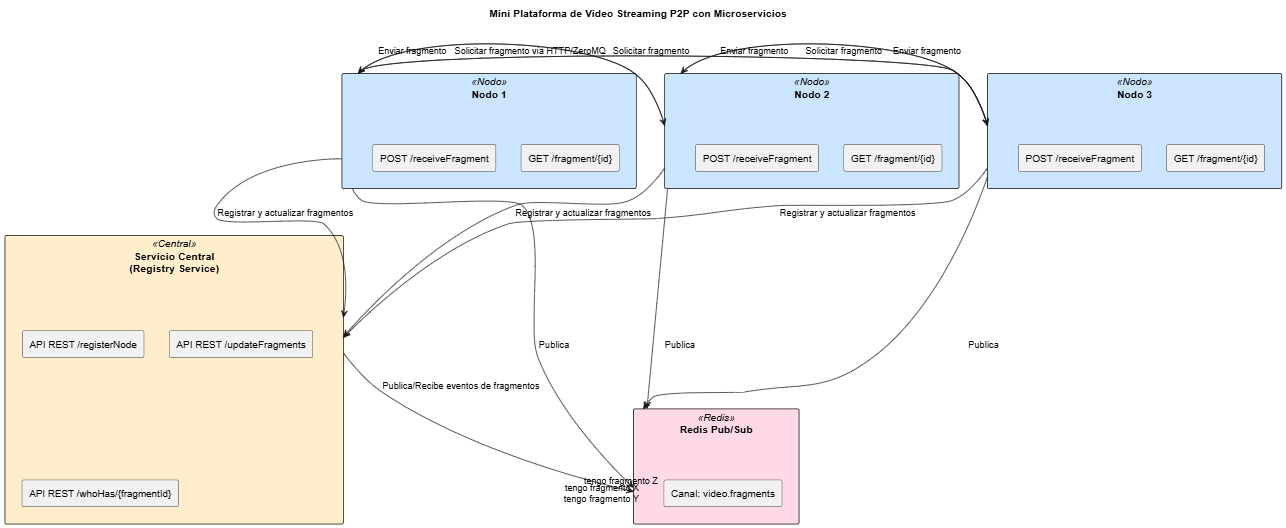
\includegraphics[width=\textwidth]{Diagramas/Diagrama.png}
\end{center}
